\documentclass[a4paper]{template/imereport}
\usepackage[utf8]{inputenc}
\usepackage{ucs}
\usepackage[ngerman]{babel}
\usepackage{graphicx}
\usepackage{wrapfig}
\usepackage{listings}
\usepackage[T1]{fontenc}
\usepackage[scaled]{beramono}

\usepackage{color}
\definecolor{bluekeywords}{rgb}{0.08,0.08,0.5}
\definecolor{greencomments}{rgb}{0,0.5,0}
\definecolor{redstrings}{rgb}{0.9,0,0}
\lstset{ %
    captionpos=b,
    breaklines=true,
    basicstyle=\footnotesize\ttfamily,
    frame=single,
    keywordstyle=\color{bluekeywords}\bfseries,
    morekeywords={proc, pure, ensures, requires, call, in, out, var, const ,init, fun, copy, ref, while, returns}
}

\pagestyle{myheadings}
\markboth{HTML Mail Filter}{HTML Mail Filter}

% Title section
\author{Florian Lüscher, Matthias Brun\\
Fachhochschule Nordwestschweiz\\
\small{\texttt{<\{florian.luescher,matthias.brun\}@students.fhnw.ch>}}
}
\title{HTML EMail Filter: Santizize Html Mails}

\begin{document}

\maketitle

% Einleitung
Obwohl in den vergangenen Jahrzehnten im Bereich des Softwareengineerings viel 
Aufwand in das Entwickeln von Technologien zur effizienteren Entwicklung robuster
Software gesteckt wurde, gibt es noch immer wenige Programmiersprachen welche 
das Schreiben robuster Software beim Sprach-Design berücksichtigt haben. Eine der Ausnahmen 
ist die Sprache Eiffel, welche beispielsweise das Definieren von Pre-/Postconditions
ermöglicht. Jedoch gibt es vermehrt auch Frameworks für etabliertere Sprachen, welche 
es erlauben, Elemente des Design-by-Contract anzuwenden und vom Compiler zu überprüfen.
In der Sprache C\# von Microsoft beispielsweise wird dies mittels \textit{Code Contracts}
 ermöglicht, welche auch vom Compiler statisch analysiert werden \cite{MS:CodeContracts}.
Auf der Java Platform gibt es über den Community Process Anstrengungen, über Annotationen
zusätzliche Metainformationen bereitszustellen, welche von einem externen Tool (z.B. FindBugs) statisch analysiert 
werden können und den Programmierer bei möglichen Fehlern warnen \cite{JSR:305}. Jedoch wurde dies
auch im aktuellen Compiler der Java Version 7 noch nicht implementiert werden. In diesem Bericht werden Erweiterungen
der Unterrichtsprache IML beschrieben, welche das Schreiben robuster Software erleichtern sollen.



% Inhalt
\section{Architektur}

Dieses Kaptitel erläutert den Aufbau unserer Applikation.
Auf der Abbildung \ref{fig:overview} sind die Klassen und Interfaces der Applikation ersichtlich. 

\begin{figure}[ht]
	\begin{center}
		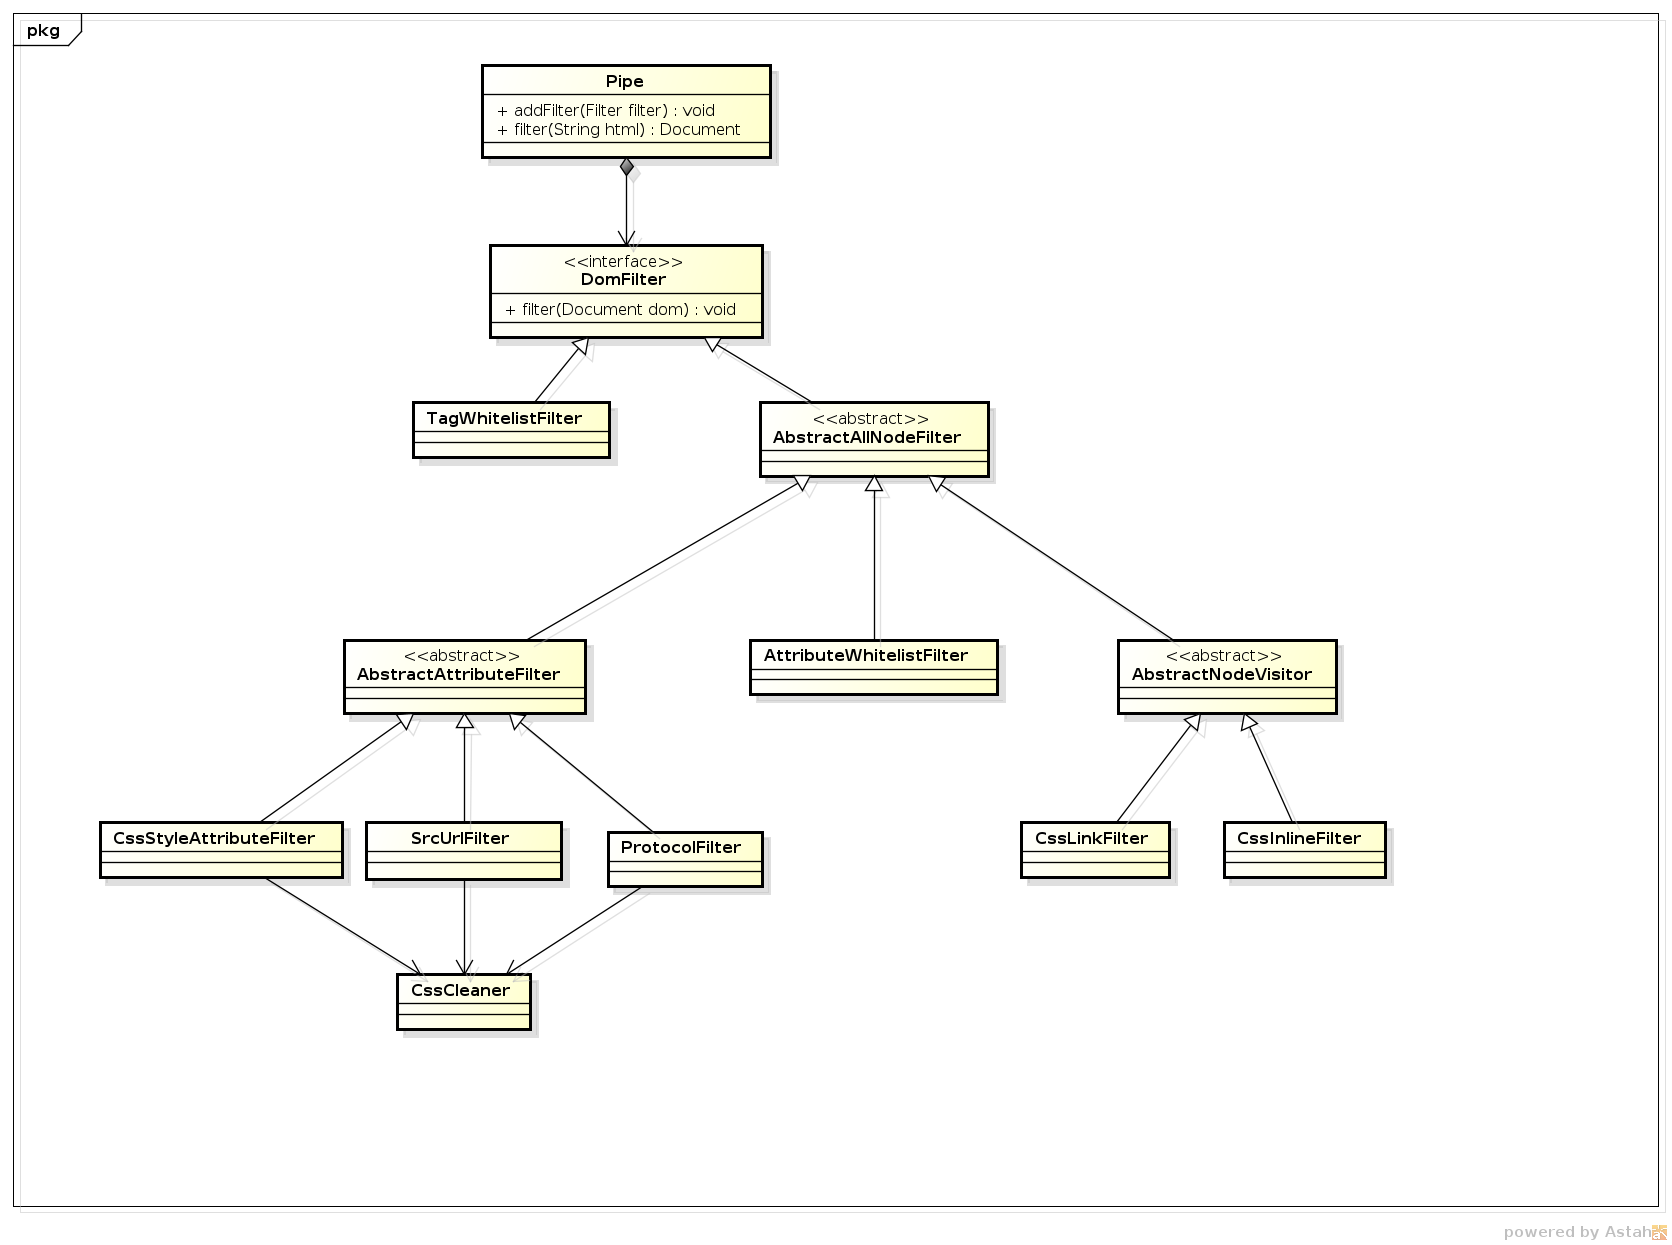
\includegraphics[width=1.0\textwidth]{./content/Class_Overview.png}
	\end{center}
	\caption{Übersicht über die Klassen und Interfaces}
	\label{fig:overview}
\end{figure}

\subsection{Verarbeitungsprozess}

Das Aktivitätsdiagramm Abbildung \ref{fig:process} beschreibt den Verarbeitungsprozess vom Starten der Applikation, bis zur Ausgabe des gesäuberten HTML Codes.

\begin{figure}[ht]
	\begin{center}
		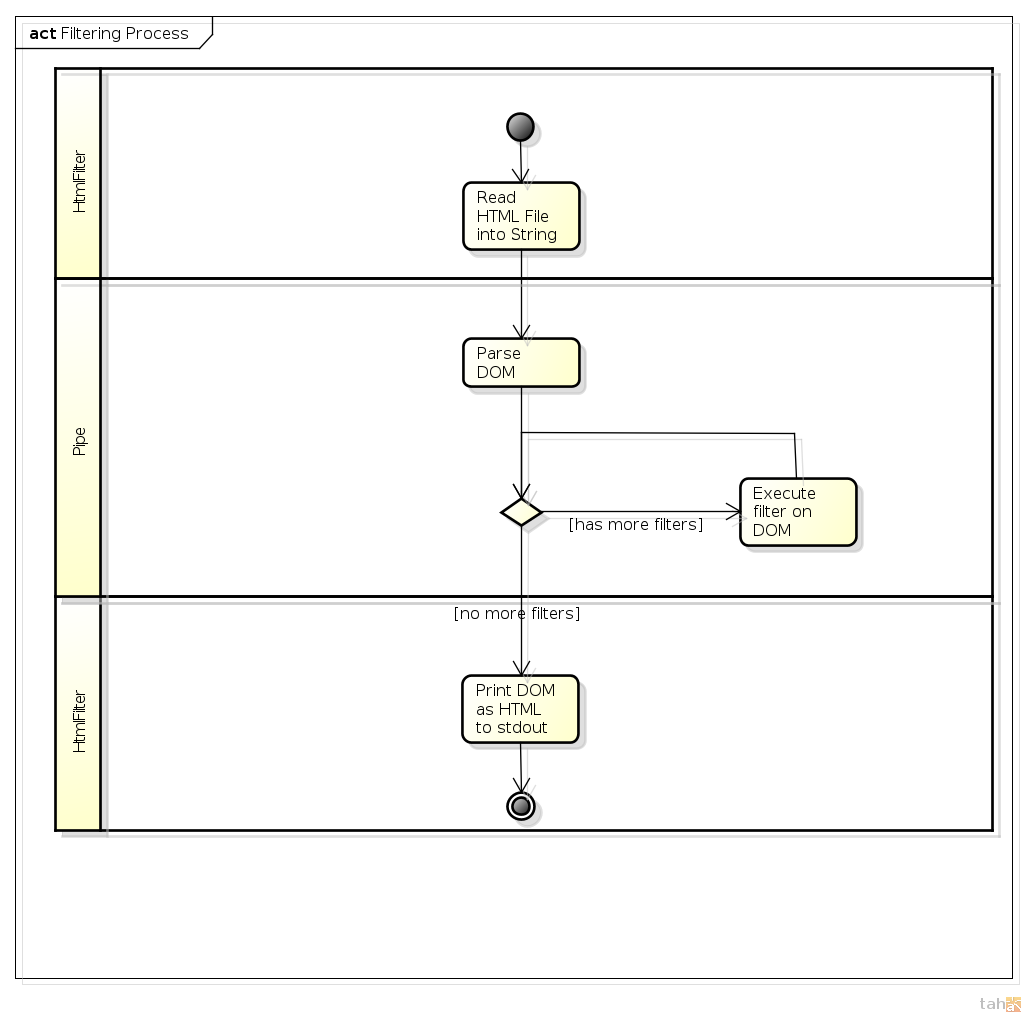
\includegraphics[width=1.0\textwidth]{./content/Filtering_Process_cut.png}
	\end{center}
	\caption{Verarbeitungsprozess}
	\label{fig:process}
\end{figure}

\newpage

\subsection{Filter}

Dieser Abschnitt beschreibt die implementierten Filter. 
In der Tabelle \ref{tab:filter} sind die implementierten Filter beschrieben.

\begin{table}[h!]
\begin{center}
\begin{tabular}{l p{10.5cm} }
\hline
\textbf{Filter} & \textbf{Beschreibung} \\ \hline \hline
TagWhitelistFilter & Dieser Filter entfernt alle HTML Tags welche nicht in der Whitelist enthalten sind. 
Beim Entfernen eines HTML Tags werden auch die zugehörigen HTML Child Nodes entfernt. \\ 

AttributeWhitelistFilter & Der Attribute Whihtelist Filter entfernt alle HTML Attribute welche nicht in der Whitelist enthalten sind. \\

ProtocolFilter & Der Protocol Filter setzt bei den HTML Attributen href und src den Wert auf "", wenn das Protokoll nicht in der Whitelist vorhanden ist. \\

SrcUrlFilter & Dieser Filter entfernt den Query Parameter beim HTML src Attribut aus der URL. Dies verhindert z.B. folgende URLs http://www.test.com/test.php?somevariables=maliciouscode in img Tags. \\

CssCleaner & Dies ist kein Filter, wird aber von Css Filter Klassen verwendet. Der CssCleaner entfernt mit Hilfe von Regular Expressions -moz-binding, behavior, @import, expression und url Tags. \\

CssStyleAttributeFilter & Dieser Filter verwendet den Css Cleaner und entefernt bei allen HTML Style Attributen die oben beschriebenen CSS Tags. \\

CssInlineFilter & Dieser Filter verwendet ebenfalls den Css Cleaner und wird bei allen HTML Style Tags angewendet. \\

CssLinkFilter & Dieser Filter entfenrt alle HTML Link Tags welche auf ein externes CSS File verweisen. \\

\hline \hline
\end{tabular}
\caption{Filter}
\label{tab:filter}
\end{center}
\end{table}

\section{Vorgehen}

In diesem Kapitel wird das Vorgehen bei der Entwicklung erläutert.

\subsection{FindBugs}

Während der gesamten Entwicklung wurde FindBugs verwendet, um mögliche Fehler bereits 
früh identifizieren zu können. Am Ende der Entwicklung meldete Findbugs keinerlei Fehler mehr.

\subsubsection{JSR-305}

Um FindBugs die Arbeit zu erleichtern, haben wir im gesamten Sourcecode die Annotationen aus dem JSR-305 
verwendet.

\subsection{Robust Programming}

Bei der Entwicklung wurde Wert darauf gelegt, Robuste Java Klassen zu entwickeln. Aus diesem Grund 
sind alle Klassen, welche nicht zur Ableitung gedacht sind \textit{final}. Bei den Abstrakten Klassen,
welche zur Ableitung designt sind, sind alle Methoden \textit{final}, die nicht von Subklassen überschrieben
werden sollen. Bei allen Klassen wurde die Sichtbarkeit der Felder minimiert, sowie auf innere Klassen 
verzichtet, um die Sichbarkeitseinschränkung nicht zu umgehen. Wenn immer möglich, wurden die 
Konstruktoren \textit{private} deklariert, und Factory-Methoden implementiert. Dies ist insbesondere
bei den Filter implementierungen zu sehen, welche meistens eine \textit{createDefault} Methode 
bereitstellen.



% Schluss
\section{Weitere Arbeiten}

Was noch verbessert werden kann..



\vspace{50pt}

\vspace{20pt}

% Quellverzeichnis
\bibliographystyle{IEEEtran}
\bibliography{report.bib}

\end{document}
